
\section{Experiments}
\label{sec:exp}

In this section, we conduct a series of experiments to empirically validate the effectiveness of our In-Place TTT framework. Specifically, we aim to answer the following research questions:

\begin{itemize}[leftmargin=8pt]

\item \textbf{Q1}: How effectively can In-Place TTT enhance pre-trained LLMs in a ``drop-in" manner?
\item \textbf{Q2}: When trained from scratch, how does In-Place TTT compare against prior TTT approaches?
\item \textbf{Q3}: What are the effects of key design choices in our In-Place TTT framework?
\end{itemize}

Using language modeling tasks of various scales as a practical proxy, we answer each question with carefully designed experiments in the following sub-sections. Due to space limits, we present detailed descriptions of experimental settings in Appendix \ref{app:exp}.

\begin{table}[!h]
\centering
\caption{Evaluation results on RULER~\citep{hsieh2024ruler}. Average accuracy (\%) is reported, with the best results in \textbf{bold}.}
\renewcommand{\arraystretch}{1.2}
\setlength{\tabcolsep}{3pt} 
\sisetup{detect-weight=true, detect-family=true}
\begin{tabular}{l S[table-format=2.2] S[table-format=2.2] S[table-format=2.2] S[table-format=2.2] S[table-format=2.2] S[table-format=2.2] | S[table-format=2.2]}
\toprule
& \multicolumn{6}{c}{In-Domain Evaluation} & \multicolumn{1}{c}{Extrapolation} \\
\cmidrule(r){2-7} \cmidrule(l){8-8}
\multicolumn{1}{c}{Model} & {4k} & {8k} & {16k} & {32k} & {64k} & {128k} & {256k} \\
\midrule
Mistral-7B~\citep{jiang2023mistral7b} & 93.6 & 91.2 & 87.2 & 75.4 & 49.0 & 13.8 & {-} \\
GLM3-6B~\citep{glm2024chatglmfamilylargelanguage}	& 87.8 & 83.4 & 78.6 & 69.9	 & 56.0 & 42.0 & {-} \\
Phi3-medium-14B \citep{abdin2024phi3technicalreporthighly} &	93.3 & 93.2	 & 91.1 & 86.8 & 78.6 & 46.1 & {-} \\
Llama3-8B~\citep{gradientlongcontextllama3} & 92.8 & 90.3 & 85.7 & 79.9 & 76.3 & 69.5 & {-} \\
Qwen3-4B (Instruct)~\citep{yang2025qwen3} & 95.1 & 93.6 & 91.0 & 87.8 & 77.8 & 66.0 & {-} \\
\midrule
Baseline & \bfseries 96.6 & 94.1 & 92.1 & 88.7 & 74.3 & 74.8 & 41.7 \\
In-Place TTT & 96.1 & \bfseries 95.6 & \bfseries 92.7 & \bfseries 89.3 & \bfseries 78.7 & \bfseries 77.0 & \bfseries 43.9 \\
\bottomrule
\end{tabular}
\label{tab:ruler128k_longct}
\end{table}

\subsection{In-Place TTT as a Drop-in Enhancement for Pre-trained LLMs}
\label{sec:exp_continual_pretrain}

To validate In-Place TTT as a ``drop-in'' enhancement for existing, pre-trained LLMs, we start with the competitive open-sourced \textit{Qwen3-4B-Base} model. Its original context window is 32k, thereby we can simulate the long-horizon, evolving tasks requiring Test-Time Training capabilities by language modeling tasks of varying context lengths. In particular, we compare the performance of (1) \textit{Qwen3-4B-Base} (Baseline); (2) \textit{Qwen3-4B-Base + In-Place TTT} (In-Place TTT). Both models undergo the exact same continual training curriculum, ensuring a fair comparison where our In-Place TTT is the only variable.

\textbf{Training and Evaluation.} The continual training curriculum is divided into two stages: an initial phase of $\sim$20B tokens with 32k context length, followed by a second phase of $\sim$15B tokens with 128k context length. The detailed descriptions of training dataset can be found in Appendix~\ref{app:dataset}. To effectively manage these long sequences, we adapt the model's Rotary Position Embeddings using YaRN~\citep{peng2023yarn}. We evaluate the long-context performance of both models on the RULER benchmark~\citep{hsieh2024ruler} using the popular OpenCompass framework~\citep{2023opencompass}, with context lengths ranging from 4k to 256k. The 256k setting specifically measures the models' ability to extrapolate beyond the 128k context length limit. Detailed descriptions of training details can be found in Appendix~\ref{app:train}.

\textbf{Results and Discussion.} The results, summarized in \cref{tab:ruler128k_longct}, demonstrate that In-Place TTT significantly boosts the long-context proficiency of the pre-trained model. In particular, a clear trend can be easily seen from the results: while both models are competitive at short contexts, Qwen3-4B-Base enhanced by our In-Place TTT establishes a consistent and widening advantage as the sequence length increases. It achieves substantial gains at the 64k and 128k context lengths. Crucially, this advantage is maintained when extrapolating to a 256k context, demonstrating superior generalization. These findings confirm that In-Place TTT can be seamlessly integrated into a pre-trained LLM to boost its long-context proficiency. The model's strong performance at and beyond the context length validates our method as a practical and powerful tool for extending the capabilities of existing LLMs.

\textbf{Extension to More Models.}
To verify the generality of our approach, we further apply In-Place TTT as a drop-in enhancement to two additional models: LLaMA-3.1-8B~\citep{grattafiori2024llama} and Qwen3-14B-Base~\citep{yang2025qwen3}, following the same continual training protocol. As shown in Table~\ref{tab:extension}, In-Place TTT consistently improves the RULER scores across all context lengths on both models. The gains are particularly pronounced at longer contexts, e.g., +2.1 at 64k for LLaMA-3.1-8B and +2.7 at 64k for Qwen3-14B-Base. Moreover, the improvement is maintained when combined with YaRN~\citep{peng2023yarn} for position extrapolation, confirming that our method is orthogonal to RoPE extension techniques. These results, spanning different model families and scales (4B--14B), reinforce that In-Place TTT is a broadly applicable drop-in enhancement for pre-trained LLMs.

\begin{table}[t]
\centering
\caption{Extension of In-Place TTT to LLaMA-3.1-8B and Qwen3-14B-Base on the RULER benchmark. We report the average accuracy (\%) with the best results in \textbf{bold}.}
\label{tab:extension}
\vspace{2mm}
\small
\begin{tabular}{llcccccc}
\toprule
Base Model & Method & 4k & 8k & 16k & 32k & 64k & 64k+YaRN \\
\midrule
\multirow{2}{*}{LLaMA-3.1-8B}
 & Baseline       & 93.9 & 92.1 & 92.5 & 91.1 & 81.6 & -- \\
 & In-Place TTT   & \textbf{94.4} & \textbf{93.0} & \textbf{93.3} & \textbf{91.7} & \textbf{83.7} & -- \\
\midrule
\multirow{2}{*}{Qwen3-14B}
 & Baseline       & 96.8 & 95.0 & 94.6 & 90.7 & 67.9 & 81.3 \\
 & In-Place TTT   & \textbf{97.2} & \textbf{95.7} & \textbf{95.2} & \textbf{91.2} & \textbf{70.6} & \textbf{82.5} \\
\bottomrule
\end{tabular}
\end{table}

\subsection{Pre-training from Scratch: A Comparative Analysis}
\label{sec:exp_from_scratch}

\begin{figure}[!h]
\centering
\begin{subfigure}[t]{0.48\textwidth}
 \captionsetup{position=top}
  \caption*{(a) Sliding Window Perplexity of 500M Model}
 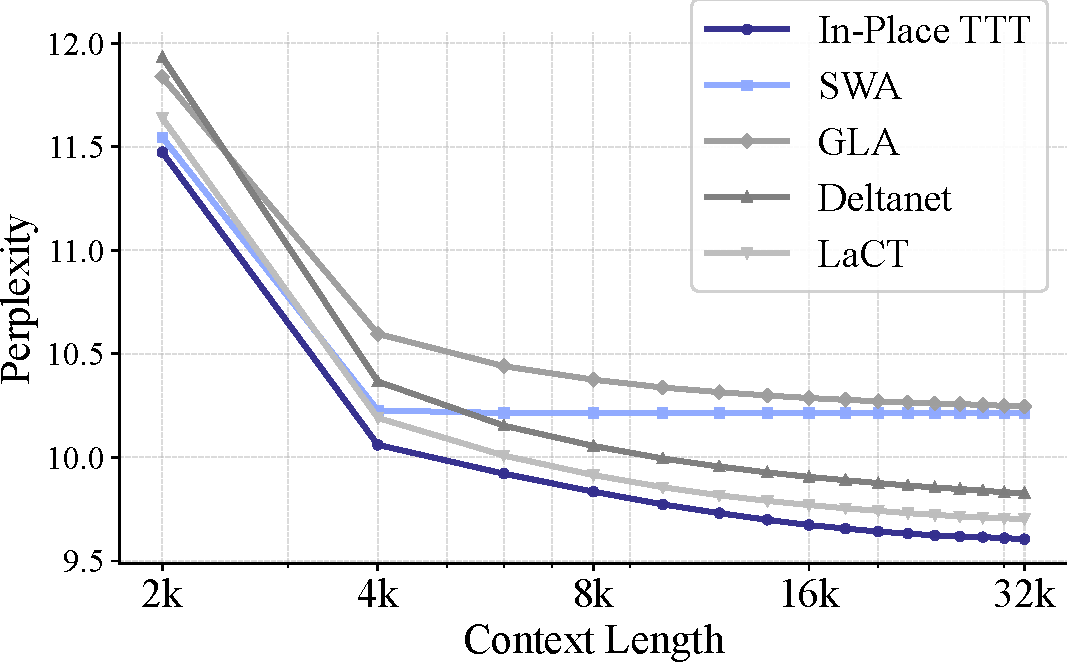
\includegraphics[width=\linewidth]{image/ttt_results_500M.pdf}
 \end{subfigure}\hfill
 \begin{subfigure}[t]{0.48\textwidth}
 \captionsetup{position=top}
 \caption*{(b) Sliding Window Perplexity of 1.5B Model}
 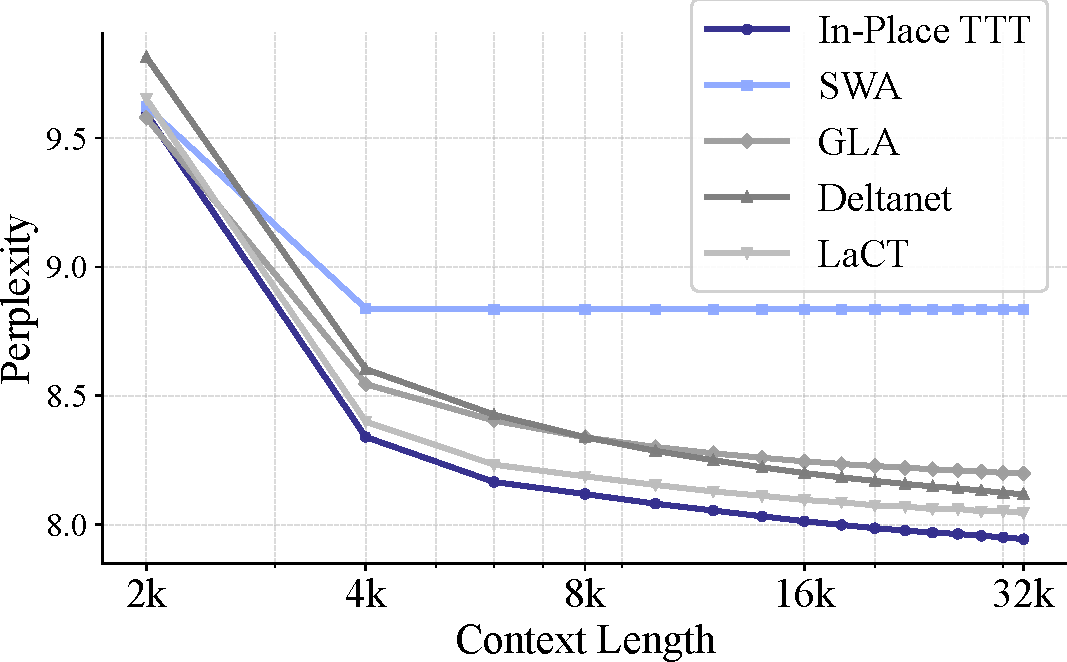
\includegraphics[width=\linewidth]{image/ttt_results_1.5B.pdf}
\end{subfigure}

 \caption{Sliding Window Perplexity at varying context lengths on the Pile dataset for 500M (left) and 1.5B (right) parameter models. Our In-Place TTT consistently achieves lower perplexity than all competitive baselines.}
  \label{fig:val-loss-500m-2b}

\end{figure}

\begin{table}[!h]
\centering
\setlength{\tabcolsep}{2pt} 
\resizebox{\textwidth}{!}{\renewcommand{\arraystretch}{1.2}
\sisetup{detect-weight=true, detect-family=true}
\begin{tabular}{ll *{5}{S[table-format=2.2]} *{3}{S[table-format=2.2]}}
\toprule
& & \multicolumn{5}{c}{Common Sense Reasoning} & \multicolumn{3}{c}{Long-Context Evaluation} \\
\cmidrule(r){3-7} \cmidrule(l){8-10}
\multicolumn{2}{c}{Model Architecture} & {HellaSwag} & {ARC-E} & {ARC-C} & {MMLU} & {PIQA} & {RULER-4k} & {RULER-8k} & {RULER-16k} \\
\midrule
\multirow{2}{*}{Baselines} & Full Attn.& 55.67 & 64.52 & 33.19 & 36.43 & 72.63 & 45.77 & 38.09 & 6.58 \\
& SWA & 54.92 & 64.18 & 32.85 & 36.06 & 72.58 & 14.77 & 9.91 & 5.07 \\
\midrule
\multirow{2}{*}{I.P. TTT} & Full Attn.& \bfseries 55.85 & \bfseries 64.98 & 32.34 & \bfseries 37.42 & \bfseries 73.29 & \bfseries 49.98 & \bfseries 43.82 & \bfseries 19.99 \\
& SWA  & 55.24 & 64.60 & \bfseries 33.70 & 36.48 & 72.03 & 28.33 & 26.80 & 7.57 \\
\bottomrule
\end{tabular}}
\caption{Evaluation results of 4B models on common sense reasoning and long-context evaluation benchmarks. Best performance is in \textbf{bold}. ``SWA'' is Sliding-Window Attention, ``Full Attn.'' is Full Attention, and ``I.P. TTT'' is our In-Place TTT.}
\label{tab:4b_results}
\end{table}



Having demonstrated In-Place TTT's effectiveness as a ``drop-in'' module, we further evaluate its performance and scalability when integrated into models pre-trained from scratch. Our analysis proceeds in two stages: we first establish its language modeling capabilities at the 500M and 1.5B scales, and then assess its scalability and impact on a larger 4B model.

\textbf{Experimental Setup.}
Firstly, we benchmark our In-Place TTT against prior TTT-related approaches and efficient attention methods based on \citet{long_data_collection} at 500M and 1.5B parameter scales. Various competitive baselines are compared: (1) standard Transformer with sliding window attention (SWA)~\citep{child2019generating,beltagy2020longformer} (2) Gated Linear Attention (GLA)~\citep{yang2024gated}; (3) DeltaNet~\citep{schlag2021linear,yangparallelizing,yang2024gdn} (4) Large Chunk Test-Time Training (LaCT)~\citep{zhang2025tttdr}. For a fair comparison, both In-Place TTT and LaCT are built upon an SWA backbone. All models are trained on sequences with a 32k context length.

Building on these results, we further scale up to 4B-parameter models to evaluate scalability of our In-Place TTT approach. In particular, we compare Transformers with Full Attention and Transformers with SWA against their counterparts enhanced by our In-Place TTT. These models are trained for 120B tokens with an 8k context length. Detailed descriptions of datasets, model configurations, and training procedures are available in \cref{app:dataset,app:model,app:train}.

\textbf{Evaluation.}
\looseness=-1 For the 500M and 1.5B models, we evaluate their long-context utilization using \textit{Sliding Window Perplexity} on a validation set comprised of Pile~\citep{gao2020pile} and Proof-Pile-2~\citep{paster2023openwebmath}. This metric measures perplexity on a fixed final block of tokens when extending the preceding context, where a decreasing perplexity trend indicates effective context usage. For the 4B models, we conduct a broader evaluation on a suite of downstream tasks, including common sense reasoning benchmarks (HellaSwag~\citep{zellers2019hellaswag}, ARC \citep{allenai:arc}, MMLU \citep{hendrycks2020measuring,hendrycks2021ethics}, PIQA~\citep{bisk2019piqa}) and the long-context RULER benchmark~\citep{hsieh2024ruler}.

\textbf{Results and Discussion.}
\looseness=-1In Figure~\ref{fig:val-loss-500m-2b}, we plot the sliding window perplexity against context length for 500M/1.5B model. It can be easily seen that our In-Place TTT consistently achieves lower validation perplexity than all competitive baselines, with its performance steadily improving up to the full 32k context. This sustained improvement suggests its core mechanism successfully compresses and utilizes information from incoming context.

Moreover, the results in Table~\ref{tab:4b_results} further show that 4B-parameter Transformers with both Full Attention and SWA are consistently improved across most common sense reasoning tasks. Furthermore, models with our In-Place TTT yield superior performance on the long-context evaluation, e.g., RULER-16k score is improved from 6.58 to 19.99 for the Transformer with Full Attention and RULER-8k score is boosted from 9.91 to 26.80 for the SWA model. These substantial gains, particularly across models of various scales, establish our In-Place TTT as a highly effective and scalable approach.


\subsection{Ablation Studies: On the Impact of Key Design Choices}
\label{sec:exp_ablation}


Lastly, we conduct a series of ablation studies on RULER with a 1.7B-parameter model, providing deeper insights into our design choices. Detailed settings are presented in Appendix~\ref{app:model} and~\ref{app:train}.

\textbf{Impact of State Size.}
We first investigate how performance scales with the fast weights size, which can be controlled by varying the number of TTT-enabled layers. Figure~\ref{fig:ablation} (a) shows a clear trend that the performance of our In-Place TTT consistently improves along with the state size scaling. This confirms that larger fast weights allow the model to more effectively adapt to contextual information, which further supports our repurposing approach leveraging the large amount of MLP states.

\textbf{Impact of Chunk Size.} The chunk size $C$ in \cref{sec:inplace_ttt_framework} controls both the granularity of fast weights updating and parallelism, exposing a tradeoff between efficiency and performance. By varying the chunk size, Figure~\ref{fig:ablation} (b) shows that both $C=512$ and $C=1024$ competitively achieve better performance compared to other choices, while $C=1024$ has better efficiency.

\textbf{Impact of LM-Aligned Objective.}
Next, we delve deep into our tailored LM-Aligned objective in \cref{sec:value_and_loss}, where the target is defined as
$\hat{\mathbf{V}} = \operatorname{Conv1D}(\mathbf{X}_0) \mathbf{W}_{\mathrm{target}}$.
In particular, the $\operatorname{Conv1D}$ operator is used to yield targets containing future token information, and the $\mathbf{W}_{\mathrm{target}}$ is a projection transformation. In Figure~\ref{fig:ablation} (c), we comprehensively ablate combinations of these components. The result shows that both of them are necessary for performance guarantee, while $\operatorname{Conv1D}$ plays an essential role on long context and $\mathbf{W}_{\mathrm{target}}$ is crucial on short context. These results align with our theoretical analysis in \cref{sec:theory}, strongly supporting our motivation to derive a tailored objective for language modeling.

\textbf{Efficiency Impact of In-Place TTT.} We further study the computational overhead introduced by our In-Place TTT. In \cref{fig:efficiency}, we compare both prefill throughput and memory consumptions of with and without our In-Place TTT. The results indeed verify the efficiency of our practical implementations.

\begin{figure}[!t]
\centering
 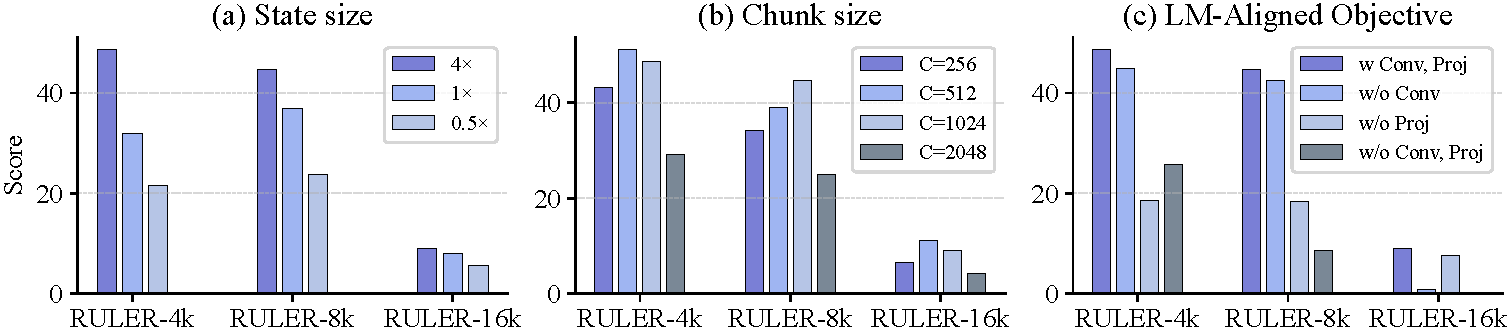
\includegraphics[width=\linewidth]{image/fig_row_preview.pdf}

 \caption{Ablation studies on the key design choices of the In-Place TTT framework, evaluated on the RULER benchmark with a 1.7B parameter model. The plots illustrate the impact of: (a) State size, showing that performance improves as the state size scales; (b) Chunk size, demonstrating a performance trade-off where intermediate sizes (e.g., 512, 1024) are optimal; and (c) The LM-Aligned Value objective, confirming that both the convolution (w Conv) and the projection (w Proj) are crucial.}
  \label{fig:ablation}
 % \vspace{-5pt}
\end{figure}

\begin{figure}[t]
\centering
\begin{subfigure}[t]{0.23\textwidth}
\captionsetup{position=top,justification=centering}
 \caption*{(a) Throughput (SWA)}
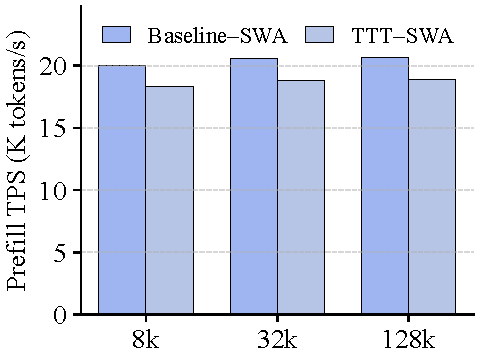
\includegraphics[width=\linewidth]{image/fig_swa_tps.pdf}
\end{subfigure}\hfill
\begin{subfigure}[t]{0.24\textwidth}
\captionsetup{position=top,justification=centering}
\caption*{(b) Throughput (Full)}
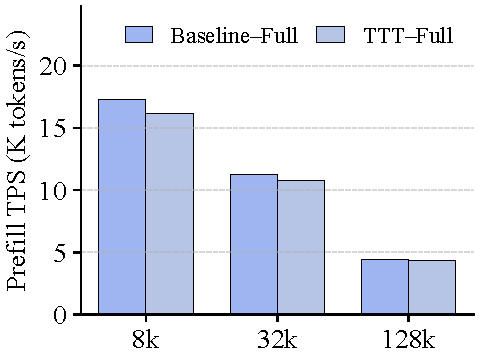
\includegraphics[width=\linewidth]{image/fig_full_tps.pdf}
\end{subfigure}\hfill
\begin{subfigure}[t]{0.24\textwidth}
\captionsetup{position=top,justification=centering}
\caption*{(c) Memory (SWA)}
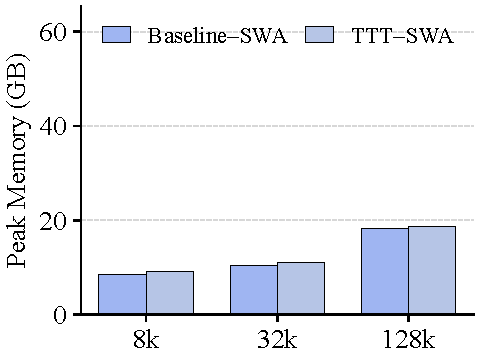
\includegraphics[width=\linewidth]{image/fig_swa_mem.pdf}
\end{subfigure}\hfill
\begin{subfigure}[t]{0.24\textwidth}
\captionsetup{position=top,justification=centering}
\caption*{(d) Memory (Full)}
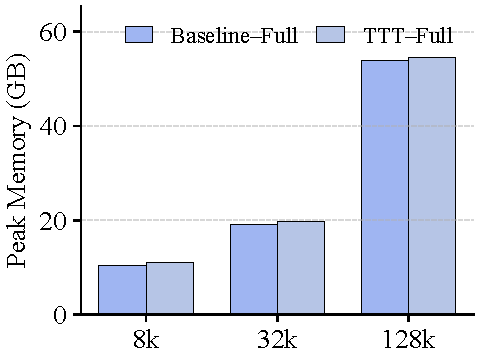
\includegraphics[width=\linewidth]{image/fig_full_mem.pdf}
\end{subfigure}

\caption{Efficiency analysis of In-Place TTT. Both prefill throughput (a, b) and peak memory (c, d) metrics are presented for 4B models with Sliding-Window Attention (SWA) and Full Attention at various context lengths. Our In-Place TTT introduces negligible overhead in practical scenarios.}
\label{fig:efficiency}

\end{figure}

\section{Related Work}
\label{app:related_work}

\textbf{Test-Time Training (TTT).}
Test-Time Training (TTT) is a paradigm that enables a model to adapt dynamically in response to continuous streams of data at inference by updating a small subset of its parameters, known as \textit{fast weights}~\citep{ba2016fastweights}. Initially demonstrating success in computer vision~\citep{sun2020ttt,wang2021tent}, TTT has since been extended to numerous other modalities—including language~\citep{sun2024tttLayers}, video~\citep{dalal2025one}, and audio~\citep{dumpala2023testtimetrainingspeech}—underscoring its broad applicability. Research in this area has largely focused on two avenues for improving TTT's effectiveness: the design of more sophisticated test-time optimizers~\citep{behrouz2025itsconnectedjourneytesttime} and the formulation of novel, self-supervised online learning objectives~\citep{behrouz2024titans,karami2025lattice}. However, the computational efficiency of TTT remained a critical bottleneck due to its inherently sequential, per-token update process. The chunk wise Test-Time Training framework was the first to directly address this challenge by introducing a chunk-wise update mechanism to better leverage parallel hardware~\citep{behrouz2024titans,irie2025fastweightprogramminglinear,zhang2025tttdr,sun2023retentive,yau2025sequentialparalleldualityprefixscannable,li2025tnt}. Despite these advances, TTT's function as the primary token mixer necessitates reliance on small chunks to preserve performance—this in turn creates a bottleneck that limits the massive parallelism needed to fully utilize modern accelerators. Furthermore, prior work has not addressed how to seamlessly integrate TTT into large, pre-trained models, nor developed learning objectives specifically tailored for the autoregressive nature of LLMs, which are gaps our work directly addresses.

\textbf{Efficient Long-Context Architectures.}
A parallel line of research seeks to extend the effective context window of LLMs by mitigating the quadratic complexity of the standard attention mechanism. Major approaches include: 1) Sparse attention methods, which restrict the range of token-to-token interactions via fixed patterns like sliding or strided windows~\citep{child2019generating,beltagy2020longformer,yuan2025nativesparseattentionhardwarealigned}; 2) Linear-time variants, which approximate the attention mechanism or replace it with efficient recurrent or gated formulations, such as linear attention \citep{katharopoulos2020linear,schlag2021linear} Gated Linear Attention (GLA)~\citep{yang2023gla}; and 3) State-Space Models (SSMs), which compress sequence history into a compact latent state, enabling processing with linear complexity~\citep{dao2023mamba,dao2024transformersssmsgeneralizedmodels}. Recently, the \textit{delta rule} has emerged as a popular design choice for linear attention and SSMs, enabling better experessivity and highly parallelizable implementations~\citep{yang2024delta}.
These architectural advances are complementary to our framework. While they focus on efficiently \textit{processing} long contexts, TTT provides a mechanism for online \textit{adaptation} to the information within that context. Our In-Place TTT can be also naturally integrated with these efficient backbones, as they also have MLP blocks. And we leave these as the future work.


\textbf{Memory Design and Augmentation.}
A related domain of research involves augmenting neural architectures with explicit memory modules to enhance their reasoning and contextual understanding capabilities. These approaches can be broadly distinguished by their function: some are designed to store persistent, task-agnostic knowledge in an external memory bank, while others focus on capturing transient, data-dependent information from the immediate context~\citep{khandelwal2019knnlm,guu2020realm,lewis2020rag,wang2024memoryllmselfupdatablelargelanguage,yu2025memagent}. The latter, contextual memories, have been implemented using various mechanisms, including recurrent state transitions, attention-based context aggregation in Transformers~\citep{dai2019transformerxl}, and rapid, gradient-based updates to fast weights~\citep{yang2024delta}. Test-Time Training (TTT) represents a powerful instance of this latter category, which conceptually extends the notion of a hidden state found in Recurrent Neural Networks (RNNs). Rather than compressing contextual history into a fixed-size activation vector, TTT designates a subset of the model's own parameters—the \textit{fast weights}—to function as a high-capacity, dynamic memory~\citep{ba2016fastweights,schlag2021linear}. These weights are updated on the fly at inference time, allowing the model to continuously internalize evolving contextual information and thereby function as an expressive, online evolving state.

\section{Conclusion}
We introduced In-Place Test-Time Training, a practical framework that resolves the critical barriers of TTT for LLMs. Principled design choices are proposed including an in-place mechanism that repurposes existing MLP blocks, an efficient chunk-wise update rule, and a theoretically-grounded objective aligned with language modeling. Extensive experiments validate that our approach not only serves as a powerful ``drop-in" enhancement for pre-trained LLMs but also outperforms strong baselines when trained from scratch. By providing a scalable solution for on-the-fly adaptation, our work makes a promising step towards a new paradigm of more dynamic, continual learning for LLMs.